\section{Project Management}\label{sec:projectManagement}
This section contains information about the project management details during the project.
\newpage
\subsection{Stakeholder}
Stakeholder Management involves identifying parties that are involved in the project. This ranges from people that are actively part of the development of the project or companies that might be interested in the end result. In the table \ref{tab:stakeholder} the most important stakeholders can be found. The stakeholders will themselves will be further explained in sections \ref{sssec:internalStakeholders}, which will explain the internal stakeholders, and \ref{sssec:externalStakeholders} will explain the external stakeholders involved in the project.
\begin{table}[htbp]
\centering
\resizebox{\textwidth}{!}{
\begin{tabular}{|p{.04\textwidth}|p{.22\textwidth}|p{.115\textwidth}|p{.118\textwidth}|p{.1\textwidth}|p{.085\textwidth}|p{.16\textwidth}|}
\hline
\textbf{Nr} & \textbf{Stakeholder} & \textbf{Company / Institution} & \textbf{Internal / External} & \textbf{Level of Interest} & \textbf{Level of Influence} & \textbf{Potential management strategies} \\ \hline
1  & Employer             & \gls{fhtenl}        & Internal            & Medium            & High               & Keep Satisfied            \\ \hline
2  & Student Workers      & \gls{fhtenl}        & Internal            & Medium            & Low                & Keep Informed             \\ \hline
3  & Graduation Student   & \gls{fhtenl}        & Internal            & High              & High               & Key Player                \\ \hline
4  & Project Manager      & \gls{fhtenl}        & Internal            & High              & High               & Key Player                \\ \hline
5  & Company Supervisor   & \gls{fhtenl}        & Internal            & High              & High               & Key Player                \\ \hline
6  & Project Team         & \gls{fhtenl}        & Internal            & High              & High               & Key Player                \\ \hline
7 & Partner University   & \gls{hsnr}          & External            & Medium              & Low                & Keep Informed             \\ \hline
8  & Pilot Company        & KLG                   & External            & High              & High               & Key Player                \\ \hline
9  & Examiner             & \gls{fhtenl}        & External            & Low               & High               & Keep Satisfied            \\ \hline
10  & Supervising Lecturer & \gls{fhtenl}        & External            & Medium            & Low                & Keep Informed             \\ \hline
\end{tabular}
}
\caption{Stakeholder Register}
\label{tab:stakeholder}
\end{table}

Figure \ref{fig:stakeholder} can be used to visualize the importance of the stakeholders. The color is used to emphasize the importance that this stakeholder is properly managed.

\begin{figure}[htbp]
	\centering
	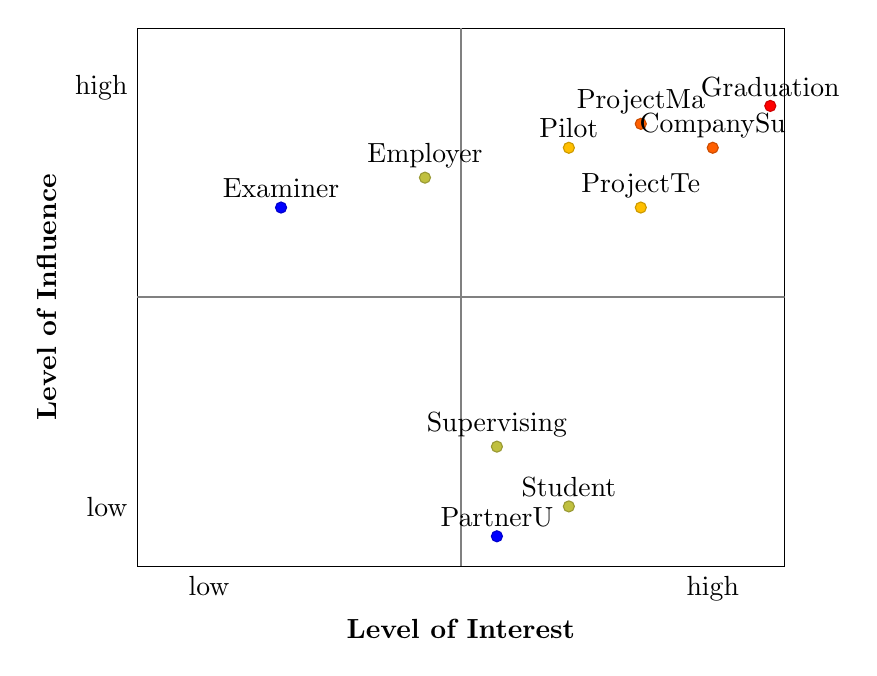
\begin{tikzpicture}
		\begin{axis}[
			scale=1.2,
			xmin=1,
			xmax=10,
			ymin=1,
			ymax=10,
			xtick,
			ytick,
			extra x ticks={2,9},
  			extra x tick labels={low, high},
  			xtick style={draw = none},
  			extra y ticks={2,9},
  			extra y tick labels={low, high},
			ytick style={draw = none},
			xlabel=\textbf{Level of Interest},
			ylabel=\textbf{Level of Influence},
			x
			]
			\addplot[
			scatter,
			only marks,
			nodes near coords*={\myvalue},  
			point meta=\thisrow{color},
			visualization depends on={value \thisrow{myvalue} \as \myvalue},
			] table[x=x, y=y]
			{
			x	y	color	myvalue
			5	7.5	2	Employer
			7	2	2	Student Workers
			7	8	3	Pilot Company 
			3	7	1	Examiner
			6	3	2	Supervising Lecturer
			9.8	8.7	5	Graduation Student 
			8	8.4	4	ProjectMa 
			9	8	4	CompanySu 
			8	7	3	ProjectTe 
			6	1.5	1	PartnerU
			};
			\addplot[gray,thick, no markers] coordinates {(1,5.5) (10,5.5)};
			\addplot[gray,thick, no markers] coordinates {(5.5,1) (5.5,10)};
		\end{axis}
	\end{tikzpicture}
	\caption{Stakeholder Graph}
	\label{fig:stakeholder}
\end{figure}
\subsubsection{Internal Stakeholders}\label{sssec:internalStakeholders}
Internal Stakeholders are parties that are a part of the team that is working directly on the project in one way or the other. In this section, the internal stakeholders mentioned in table \ref{tab:stakeholder} will be listed again and explained.

\begin{description}
	\item[Employer] \hfill
	
	The employer in this project is an institution and not a single person. This does not change the fact, that the employer is interested in the project, as he is financing the project. Also the employer could change the outcome, if he is not accepting the proposed plans. It is important, that this party is kept satisfied as more work could be created when the plan has to change.
	\item[Student Workers] \hfill
	
	Student Workers are employed to help in the LOGwear project in general. While they currently are not involved with the process of the creation of the demo facility that might change in the future, therefore they should be kept informed.
	\item[Graduation Student] \hfill
	
	The graduation student is the person mainly responsible for the development of the demo facility and therefore has a lot of responsibility and interest towards the project.
	\item[Project Manager] \hfill
	
	The project manager is responsible for the general planning of the project. Planning meetings with the different parties and coordinating them.
	\item[Company Supervisor] \hfill
	
	The company supervisor is looking over the progress of the graduation student and is giving advice if needed. 
	\item[Project Team] \hfill
	
	The project team are the members of the team actively developing the application prototype and are involved in building the demo facility afterwards.
\end{description}

\subsubsection{External Stakeholders}\label{sssec:externalStakeholders}
External Stakeholders are parties that are involved in the project, but are not a part of the team actively developing the project. In this section, the external stakeholders mentioned in table \ref{tab:stakeholder} will be listed again and explained.

\begin{description}
	\item[Partner University] \hfill
	
	The partner university is also working on the LOGwear project, but on a different aspect. They might be interested in project of creating a demo facility, but probably will not interfere with it.\\
	
	\item[Pilot Company] \hfill
	
	The pilot company involved is the logistics company KLG. They bring in the highest amount of domain knowledge and are interested in the project to improve their own processes. They could influence the project easily by not approving the planned demo facility due to problems with how the logistics process is modelled.
	\item[Examiner] \hfill
	
	While the examiner is not involved in the project itself, the examiner will finally assesses the performance of the graduation student.
	\item[Supervising Lecturer] \hfill
	
	The supervising lecturer is there to answer questions and support the student from a software engineering standpoint. While not having a lot of influence on the project itself, the supervising lecturer is interested in what the student is doing and especially how he is doing it.
\end{description}
\newpage
\subsection{Risks}
Risk management is about identifying risks and finding solutions to problems before they can occur. The list of risks can be found in table \ref{tab:RiskRegister}. The identified risks will increase as the project moves forward. Especially when a decision is made for the wearable and the process. 

\begin{table}[htbp]
\centering
\footnotesize
\resizebox{\textwidth}{!}{
\begin{tabular}{|>{\raggedright\arraybackslash}p{.03\textwidth}|>{\raggedright\arraybackslash}p{.1\textwidth}|>{\raggedright\arraybackslash}p{.2\textwidth}|>{\raggedright\arraybackslash}p{.08\textwidth}|>{\raggedright\arraybackslash}p{.08\textwidth}|>{\raggedright\arraybackslash}p{.15\textwidth}|>{\raggedright\arraybackslash}p{.13\textwidth}|>{\raggedright\arraybackslash}p{.11\textwidth}|}
\hline
\textbf{Nr} & \textbf{Risk Name}                                    & \textbf{Description}                                                                                                      & \textbf{Prob-ability} & \textbf{Impact} & \textbf{Root Cause}                                                                                       & \textbf{Potential Responses}                                              & \textbf{Risk Owner} \\
\hline
1           & Wearable unavailable          & The wearable desired to be used in the demo facility is unavailable.                                                      & Low                  & Medium          & The desired product is a prototype or similar.                                                            & Choosing a different wearable that is already readily available.          & Graduation Student  \\ \hline
2           & Demo Area & A demo area is in mind that could potentially be rented, but that could not be possible.                                  & Medium               & Medium          & The owner of the place does not rent the area.                                                            & Researching possible places where the demo facility could be created.     & Graduation Student  \\ \hline
3           & Unusable wearable             & A wearable is chosen that does not have the capabilities to fulfill the things that were planned with the demo facility.  & Low                  & High            & Too little research done on the wearables, or the researched material was wrong.                          & Altering the demo scenario to accommodate the problems with the wearable. & Graduation Student  \\ \hline
4           & Vocabulary unclear            & The vocabulary used in the logistics branch, especially abbreviations and acronyms might cause problems in communication. & High                 & Low             & The graduation student has too little knowledge of the logistics branch, at the beginning of the project. & Asking questions if a word's or sentence's meaning is not clear.          & Graduation Student \\ \hline
5 & Communi-cation Problems & When explaining a task, a phrase or word is understood differently from different parties. & High & Medium & The proper definition is not known to everyone and are expecting a different meaning from a given phrase or word. & When the misunderstanding is discovered the different parties talk out what is expected from that term and come to a common understanding. & Project Team \\ \hline
\end{tabular}
}
\caption{Risk Register}
\label{tab:RiskRegister}
\end{table}

\begin{wrapfigure}{l}{0pt}
	\centering
	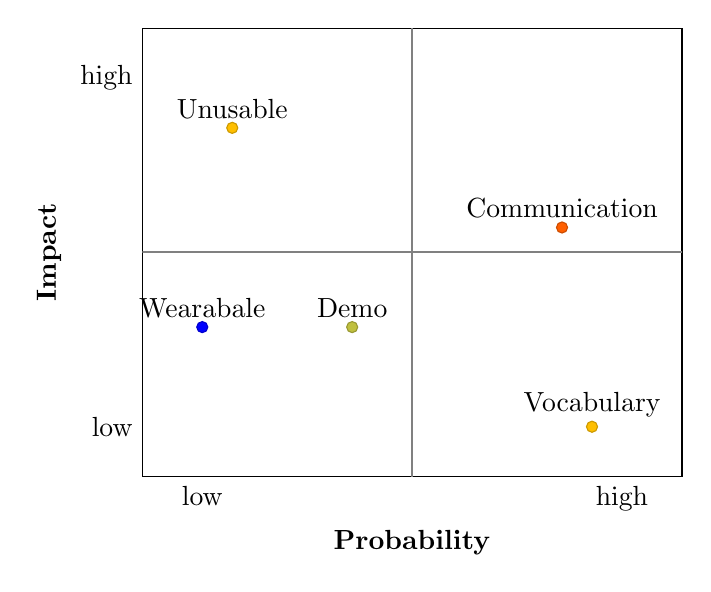
\begin{tikzpicture}
		\begin{axis}[
			scale=1,
			xmin=1,
			xmax=10,
			ymin=1,
			ymax=10,
			xtick,
			ytick,
			extra x ticks={2,9},
  			extra x tick labels={low, high},
  			xtick style={draw = none},
  			extra y ticks={2,9},
  			extra y tick labels={low, high},
			ytick style={draw = none},			
			xlabel=\textbf{Probability},
			ylabel=\textbf{Impact},
			x
			]
			\addplot[
			scatter,
			only marks,
			nodes near coords*={\myvalue},  
			point meta=\thisrow{color},
			visualization depends on={value \thisrow{myvalue} \as \myvalue},
			] table[x=x, y=y]
			{
			x	y	color	myvalue
			2	4	1	Wearabale
			4.5	4	2	Demo
			2.5	8	3	Unusable
			8.5	2	3	Vocabulary
			8	6	4	Communication
			0	0 	5
			};
			\addplot[gray,thick, no markers] coordinates {(1,5.5) (10,5.5)};
			\addplot[gray,thick, no markers] coordinates {(5.5,1) (5.5,10)};
		\end{axis}
	\end{tikzpicture}
	\caption{Risk Graph}
	\label{fig:risks}
\end{wrapfigure}

In figure \ref{fig:risks} the risks can be seen in a graph that shows their Probability and Impact again. The color emphasizes the amount of attention a risk should get, in order for the project to continue smoothly. The figure also shows more fine grained the probability and impact of the risks than just low, medium and high.

\cleardoublepage

\subsection{Requirements}
Requirements are for the demo facility only, as the reference model is not an actual product to have any requirements for. Of the current state the demo facility only has few requirements as the wearable is not chosen at this point and only the process is known.

\begin{table}[htbp]
\begin{tabular}{c}

\end{tabular}
\caption{Requirements}
\label{tab:requirements}
\end{table}
\subsection{Quality Management}
Metrics used to determine the quality of the project:

\begin{itemize}
	\item code coverage
	\item language conventions
	\item documentation
	\item possibly performance testing (as wearables tend to be not as powerful focus on performance might not be wrong)
	\item integration testing
	\item code reviews(?)
\end{itemize}
\subsection{Definition of Done}
A part of the software project is done, when it is fully designed, implemented and tested. When that part of the application is passing all of these criteria it is added to a repository where the result is build. When that build is successful that part of the application is done, for the moment. When that part needs to be changed in the future the same procedure will be used again.